\documentclass[11pt]{article}
\usepackage[utf8]{inputenc}
\usepackage{graphicx} % Allows you to insert figures
\usepackage{amsmath} % Allows you to do equations
\usepackage{fancyhdr} % Formats the header
\usepackage{hyperref}
\usepackage{fancyhdr}%header and footer
\pagestyle{fancy}
\fancyhead{}
\fancyfoot{}
\fancyfoot[R]{\thepage}
\usepackage[a4paper, inner=1.7cm, outer=2.7cm, top=2cm, bottom=2cm, bindingoffset=1.2cm]{geometry} % Formats the paper size, orientation, and margins
\linespread{1.25} % about 1.5 spacing in Word
\setlength{\parindent}{0pt} % no paragraph indents
\setlength{\parskip}{1em} % paragraphs separated by one line

\begin{document}

%START THE TITLE PAGE
\begin{titlepage}
\begin{center}
    
\includegraphics[width=8cm]{images/logo.jpg}
\end{center}

\begin{center}
\begin{Large}
\textbf{SOEN 6011 : SOFTWARE ENGINEERING PROCESSES} \\
\vspace*{0.1in}
\textbf{SUMMER 2022}\\
\vspace*{0.9in}
\end{Large}
\begin{Large}
\textbf{ETERNITY}\\
\vspace*{0.1in}
Instructor: PANKAJ KAMTHAN \\
\vspace*{0.9in}
\begin{Huge}
\textbf{Project Report}\\
\vspace*{0.9in}
\end{Huge}
\end{Large}

\begin{center}
    \line(1,0){300}\\
    \textbf{Student Name: Yun Ni\\
    Student ID: 40179775}\\
    \textbf{July, 2022}\\
    \line(1,0){300}\\
    \vspace*{0.5in}
    \textbf{Overleaf}:\url{https://www.overleaf.com/project/62ccdd9901199fc8cfc53a1f} \\
    \textbf{Github}: \url{https://github.com/ninanee/SOEN6011_Project} 
\end{center}
\end{center}

\end{titlepage}
%END THE TITLE PAGE

\newpage
\section{PROBLEM 1}\label{problem1}
\subsection{Introduction}
The function $f(x) = ab^x$ is an exponential function where $a\neq0, b>0$ and $b\neq1$. In this exponential function, $a$ is a initial quality, $b$ is the growth factor or decay factor and $c$ is the exponent. The function is called exponential because it has the input variable in the exponent and we can repeatedly multiplying by $b$~\cite{browder2012mathematical}.

\subsection{Domain}
The domain of this function is given by all the values that $x$ can take. If $b$ is a positive real number other than 1 and $a> 0$, $x$ can take any value.\\
Therefore, the domain is \textbf{$x\in R$}.

\subsection{Co-domain}
The co-domain is given by the dependent values of the variable $y$, where $y = ab^x$. If we evaluate $f(-\infty)$ then $y$ tends to zero. Besides, if we evaluate $f(\infty)$ then $y$ tends to infinity.
Therefore, the co-domain is $(0, \infty)$.

\subsection{Characteristics}
\begin{itemize}
    \item Growth: if $b>0$, the function represents exponential growth which is a function increasing at a constant percentage. It is shown on the right hand side of Figure \ref{fig:my_label}.
    \item Decay: if $0<b<1$, the function represents exponential decay which is a function decreasing at a constant percentage. It is shown on the left hand side of Figure \ref{fig:my_label}.
    \item Invective and Subjective: this function is subjective since for every $y$, there is an $x$ such that $f(x) = y$, and it is not an invective function.
\end{itemize}

\begin{figure}[h]
    \centering
    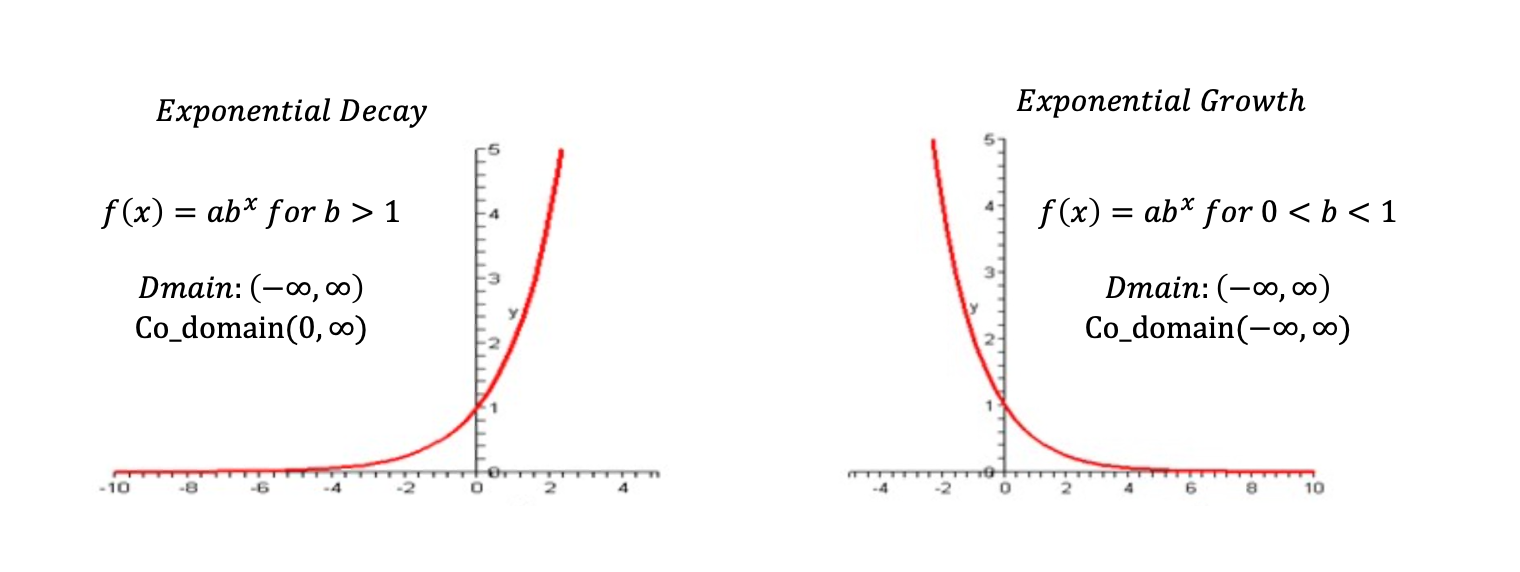
\includegraphics[width=12cm]{images/Function.png}
    \caption{The graph representation of $f(x) = ab^x$}
    \label{fig:my_label}
\end{figure}

\subsection{Context of Use Model}
The context of use model for the exponential function calculator is represented by the UML Class Diagram as Figure \ref{fig:context}.
\begin{figure}[h]
    \centering
    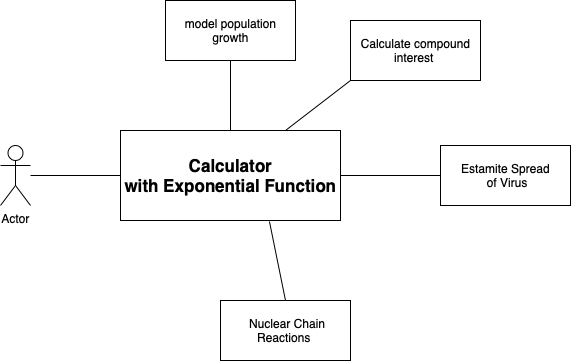
\includegraphics[width=8cm]{images/Context_diagram.png}
    \caption{The Context Diagram for exponential function calculator}
    \label{fig:context}
\end{figure}

As the figure shows above, the calculator can be used in both technical and non-technical environment \cite{zelen1966application}\cite{lebanon2001boosting}.
\begin{itemize}
    \item Technical Environment: help scientists model the number of new infections over time.
    \item Non-technical environment: help a student calculate the retirement account.
\end{itemize}

\section{PROBLEM 2}\label{problem2}
This section presents the assumptions and requirements for implementing $f(x)=ab^x$.
\subsection{Assumptions}
\begin{enumerate}
    \item The Function will accept only real numbers as inputs.
    \item The Function will be able to handle entry value of double-precision floating-point.
\end{enumerate}

\subsection{Requirements}
\begin{center}
    \begin{tabular}{|p{3cm}|p{11cm}| }
    \hline
    \textbf{Identification} &  FR1 \\ \hline 
    \textbf{Type} & Functional Requirement\\ \hline 
    \textbf{Priority} & High  \\ \hline
    \textbf{Difficulty} & Medium  \\ \hline
    \textbf{Description} & System needs to take inputs $x, a, b$ to give an output of $ab^x$. Besides, needs to define the constrains that $a\neq0, b > 0, b \neq 1$. Because, when $a=0$ or $b=0$, the function will be simplified to $y = f(x) = 0$. In addition, when $b = 1$,  the function will be simplified to $y = f(x) = a$, like a constant function.\\ \hline
\end{tabular}
\end{center}

\begin{center}
    \begin{tabular}{|p{3cm}|p{11cm}| }
    \hline
    \textbf{Identification} &  FR2 \\ \hline 
    \textbf{Type} & Functional Requirement\\ \hline 
    \textbf{Priority} & High  \\ \hline
    \textbf{Difficulty} & Medium  \\ \hline
    \textbf{Description} & Function $ab^x$ does not depend on any other functions like built-in or library functions.\\ \hline
\end{tabular}
\end{center}

\begin{center}
    \begin{tabular}{|p{3cm}|p{11cm}| }
    \hline
    \textbf{Identification} &  FR3 \\ \hline 
    \textbf{Type} & Functional Requirement\\ \hline 
    \textbf{Priority} & High  \\ \hline
    \textbf{Difficulty} & Medium  \\ \hline
    \textbf{Description} & Users can give an input from all real numbers for $x$.\\ \hline
\end{tabular}
\end{center}

\begin{center}
    \begin{tabular}{|p{3cm}|p{11cm}| }
    \hline
    \textbf{Identification} &  FR4 \\ \hline 
    \textbf{Type} & Functional Requirement\\ \hline 
    \textbf{Priority} & High  \\ \hline
    \textbf{Difficulty} & Easy  \\ \hline
    \textbf{Description} & When users give other inputs than a number like a string, the system should not accept and should show the exception properly.\\ \hline
\end{tabular}
\end{center}

\begin{center}
    \begin{tabular}{|p{3cm}|p{11cm}| }
    \hline
    \textbf{Identification} &  FR5 \\ \hline 
    \textbf{Type} & Functional Requirement\\ \hline 
    \textbf{Priority} & High  \\ \hline
    \textbf{Difficulty} & Easy  \\ \hline
    \textbf{Description} & When users give inputs does not specify all there inputs like $a, b, x$, the system should not accept and throw an error.\\ \hline
\end{tabular}
\end{center}

\begin{center}
    \begin{tabular}{|p{3cm}|p{11cm}| }
    \hline
    \textbf{Identification} &  FR6 \\ \hline 
    \textbf{Type} & Functional Requirement\\ \hline 
    \textbf{Priority} & High  \\ \hline
    \textbf{Difficulty} & Easy  \\ \hline
    \textbf{Description} &Ensure the accuracy of decimal operations to the power of decimals.\\ \hline
\end{tabular}
\end{center}

\section{PROBLEM 3}\label{problem3}
This section presents the pseudo-code and algorithm for implementing $f(x)=ab^x$.

\newpage
\bibliographystyle{plain}
\bibliography{bibliography.bib}
\end{document}